%% hf: enable header and footer.
\documentclass[
twocolumn,
% hf,
]{ceurart}

% One can fix some overfills
% \sloppy

% This was used to mitigate some warnings
\usepackage[T1]{fontenc}
\usepackage{lmodern}

\begin{document}

% Rights management information. CC-BY is the default license.
\copyrightyear{2024}
\copyrightclause{Copyright for this paper by its authors.
  Use permitted under Creative Commons License Attribution 4.0
  International (CC BY 4.0).}

\conference{BPM 2024: Demos and Resources, September 01-06, 2024, Krakow, PL}

\title{BPMN Analyzer 2.0: Instantaneous, Comprehensible, and Fixable Anomaly Detection for Realistic BPMN Models}

\author[1]{Tim Kräuter}
[email=tkra@hvl.no]
\author[1]{Patrick Stünkel}
[email=past@hvl.no] % patrick.stuenkel@hvl.no
\author[1]{Adrian Rutle}
[email=aru@hvl.no]
\author[1]{Yngve Lamo}
[email=yla@hvl.no]
\author[2,1]{Harald König}
[email=harald.koenig@fhdw.de]
\address[1]{Western Norway University of Applied Sciences, Bergen, Norway}
\address[2]{FHDW Hannover, Germany}

\begin{abstract}
% 102 words
Many business process models have control-flow anomalies, such as deadlocks or livelocks, which hinder proper execution.
In this paper, we introduce a new tool that can instantaneously identify anomalies in BPMN models, make them understandable for modelers, and suggest corrections to resolve them.
We demonstrate that detection is instantaneous by benchmarking our tool against synthetic BPMN models with increasing size and state space complexity, as well as realistic models.
Moreover, the tool directly displays detected anomalies in the model, including an interactive visualization, and suggests fixes to resolve them.
The tool is open-source, extensible, and integrated into a popular BPMN modeling tool.
\end{abstract}

\begin{keywords}
BPM,
Verification,
Control-flow Analysis,
BPMN model checking,
Soundness,
Safeness
\end{keywords}

\maketitle

% Details can be found here: https://bpm2024.agh.edu.pl/call-for-demos-and-resources/
% 5 pages including references
% Extended version on GitHub and then on Arxiv once submitted

% An introduction section, which, among others, should highlight the significance of the tool or resource to the BPM field;
\section{Introduction}
The tool is available online\footnote{\url{https://timkraeuter.com/bpmn-analyzer-js/}} alongside a video demonstration\footnote{\url{https://www.youtube.com/watch?v=MxXbNUl6IjE}}.
% Why is it significant for the BPM field?

\begin{figure}[ht]
	\centering
	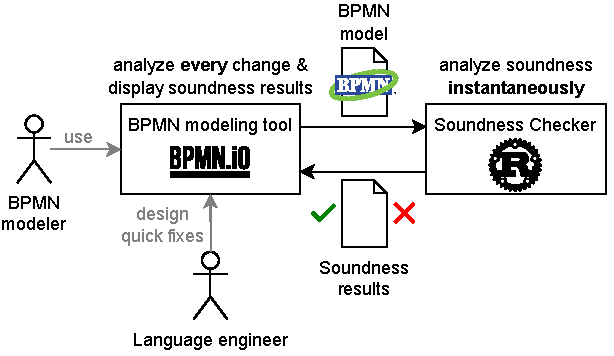
\includegraphics[width=\linewidth]{images/overview}
	\caption{Overview of the tool}
	\label{fig:overview}
\end{figure}

% Must have section according to the description
% A section discussing the innovations of the tool or resource to the BPM community and its main characteristics or features
\section{Innovations} % Main tool description and showing the innovations
Three main innovations of the tool:
% Instantaneous
% Comprehensible
% Fixable

\section{Maturity of the tool}
% Scalability tests (instantaneous)
Improves upon our previous BPMN Analyzer tool~\cite{krauterFormalizationAnalysisBPMN2023}.
% bpmn.io forum link/mention: https://forum.bpmn.io/t/automatic-bpmn-control-flow-analysis-and-resolution/11150


% \begin{acknowledgments}
% Thanks to the anonymous reviewers for their valuable feedback.
% \end{acknowledgments}

\section{Related work?}
% Could cite my other extended version and put that on arxiv.

\section{Conclusion \& future work}

In this paper, we describe a novel tool that provides instantaneous, comprehensible, and fixable BPMN control-flow anomaly detection and is integrated into a popular BPMN modeling tool.
We benchmarked our tool against synthetic and realistic BPMN models to demonstrate instantaneous soundness checking.
We address the three main challenges for providing soundness-checking capabilities to non-expert users as identified in~\cite{fahlandAnalysisDemandInstantaneous2011}.
First, a model checker must be able to check all or most user-created models, i.e., it must support the most used BPMN elements.
This is not a problem for most tools, including ours, which has similar capabilities to~\cite{corradiniFormalApproachAnalysis2021}, and we plan to increase our tool's BPMN coverage as needed.
Second, model checking must be \textit{instantaneous} since long runtimes are unacceptable and often interpreted as tool errors~\cite{fahlandAnalysisDemandInstantaneous2011}.
Third, the biggest challenge for model checking is \textit{consumability}, i.e., reporting the found violations in a comprehensible user interface.
Our tool addresses all these challenges and even provides quick fixes for common anomalies.
The tool is a BPMN-specific model checker written in Rust paired with an intuitive user interface based on the popular \textit{bpmn.io} ecosystem that allows easy extension in the future.

\bibliography{bib}

% If your work has an appendix, this is the place to put it.
% \appendix

\end{document}
